\section{Desarrollo } 

\subsection {Crear Relaciones}
\begin{itemize}
 \item 1.Conectando a Power Bi a datos
 Copiar el script Task 1 del archivo Lab Exercise1.sql. y pegar la consulta en Power BI, en el cuadro sentencia SQL.
	\begin{center}
	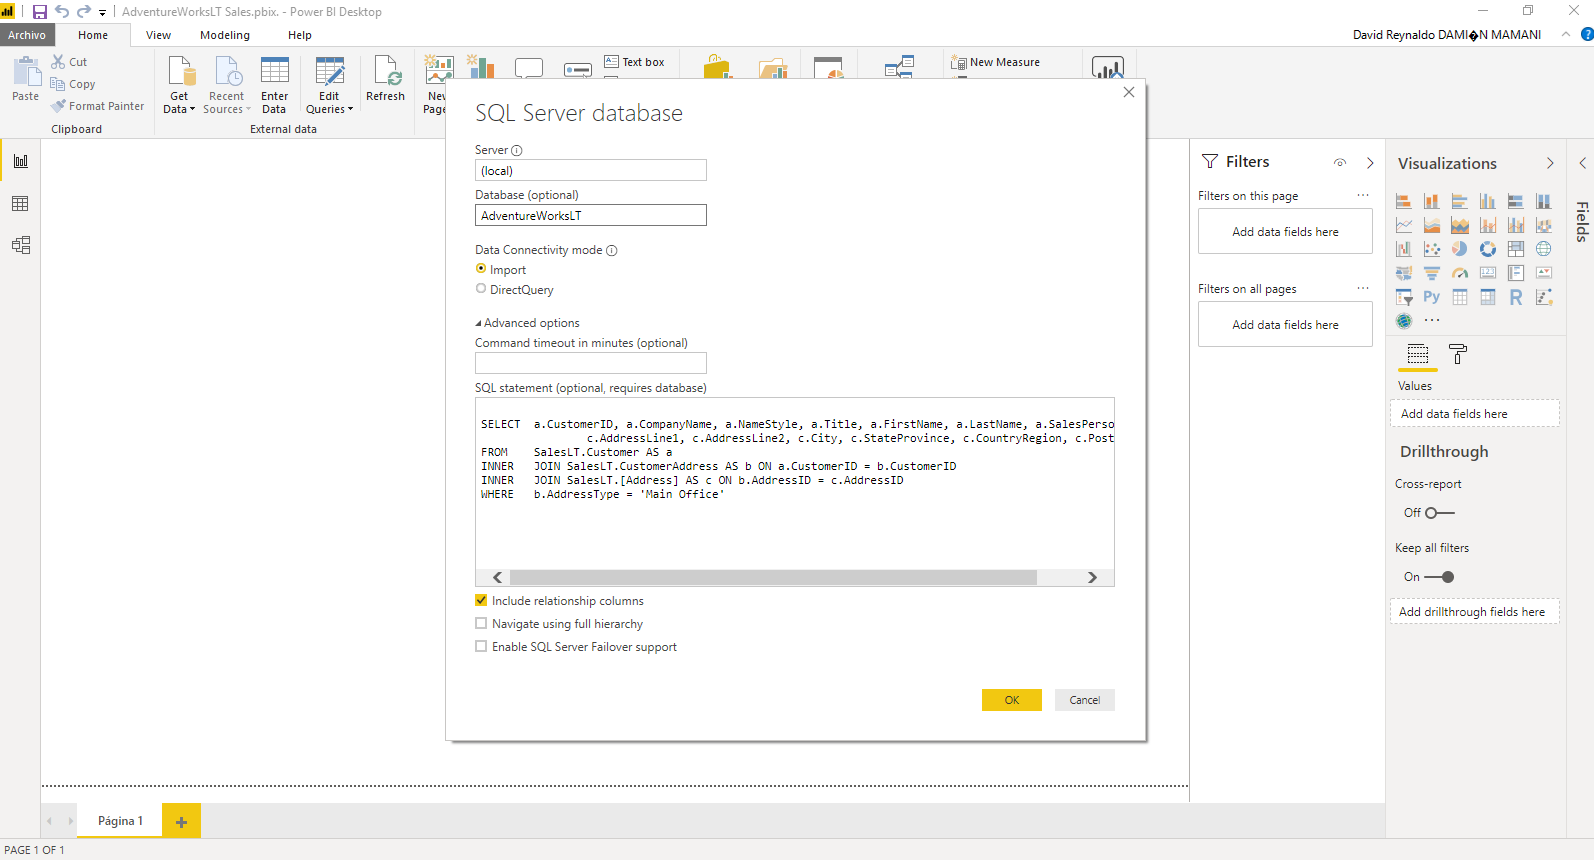
\includegraphics[width=18cm]{./Imagenes/I1}
	\end{center}	
Datos Conectados
\begin{center}
	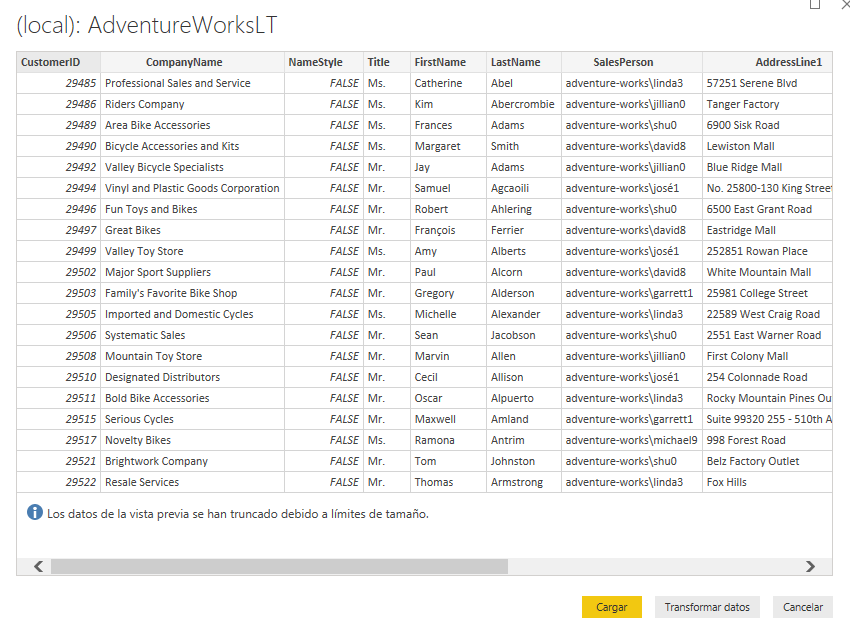
\includegraphics[width=18cm]{./Imagenes/I2}
	\end{center}	

 \item 2.Graficar Datos
Formula cambiada a English (United States). Todos los script insertados de tal manera que nos da los siguientes valores.
	\begin{center}
	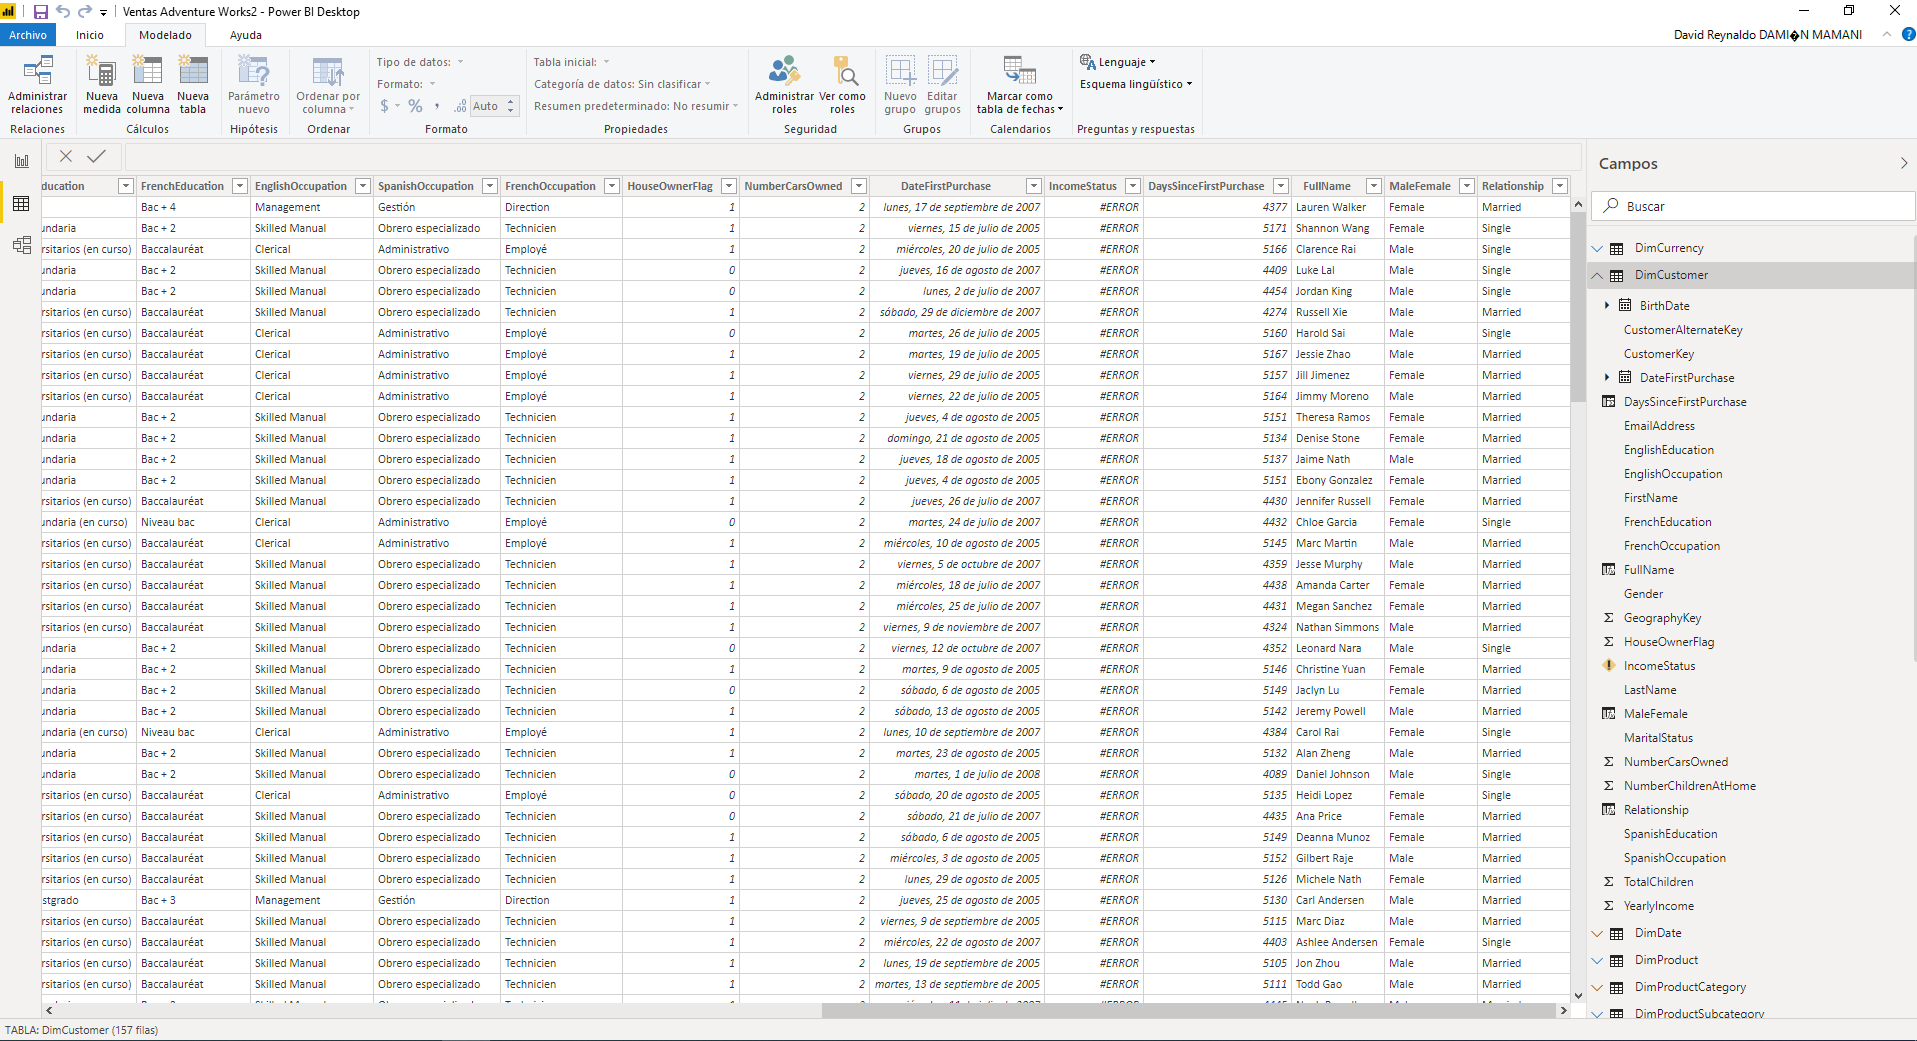
\includegraphics[width=18cm]{./Imagenes/Imagen3}
	\end{center}	

 \item 3.Combinar Data

	\begin{center}
	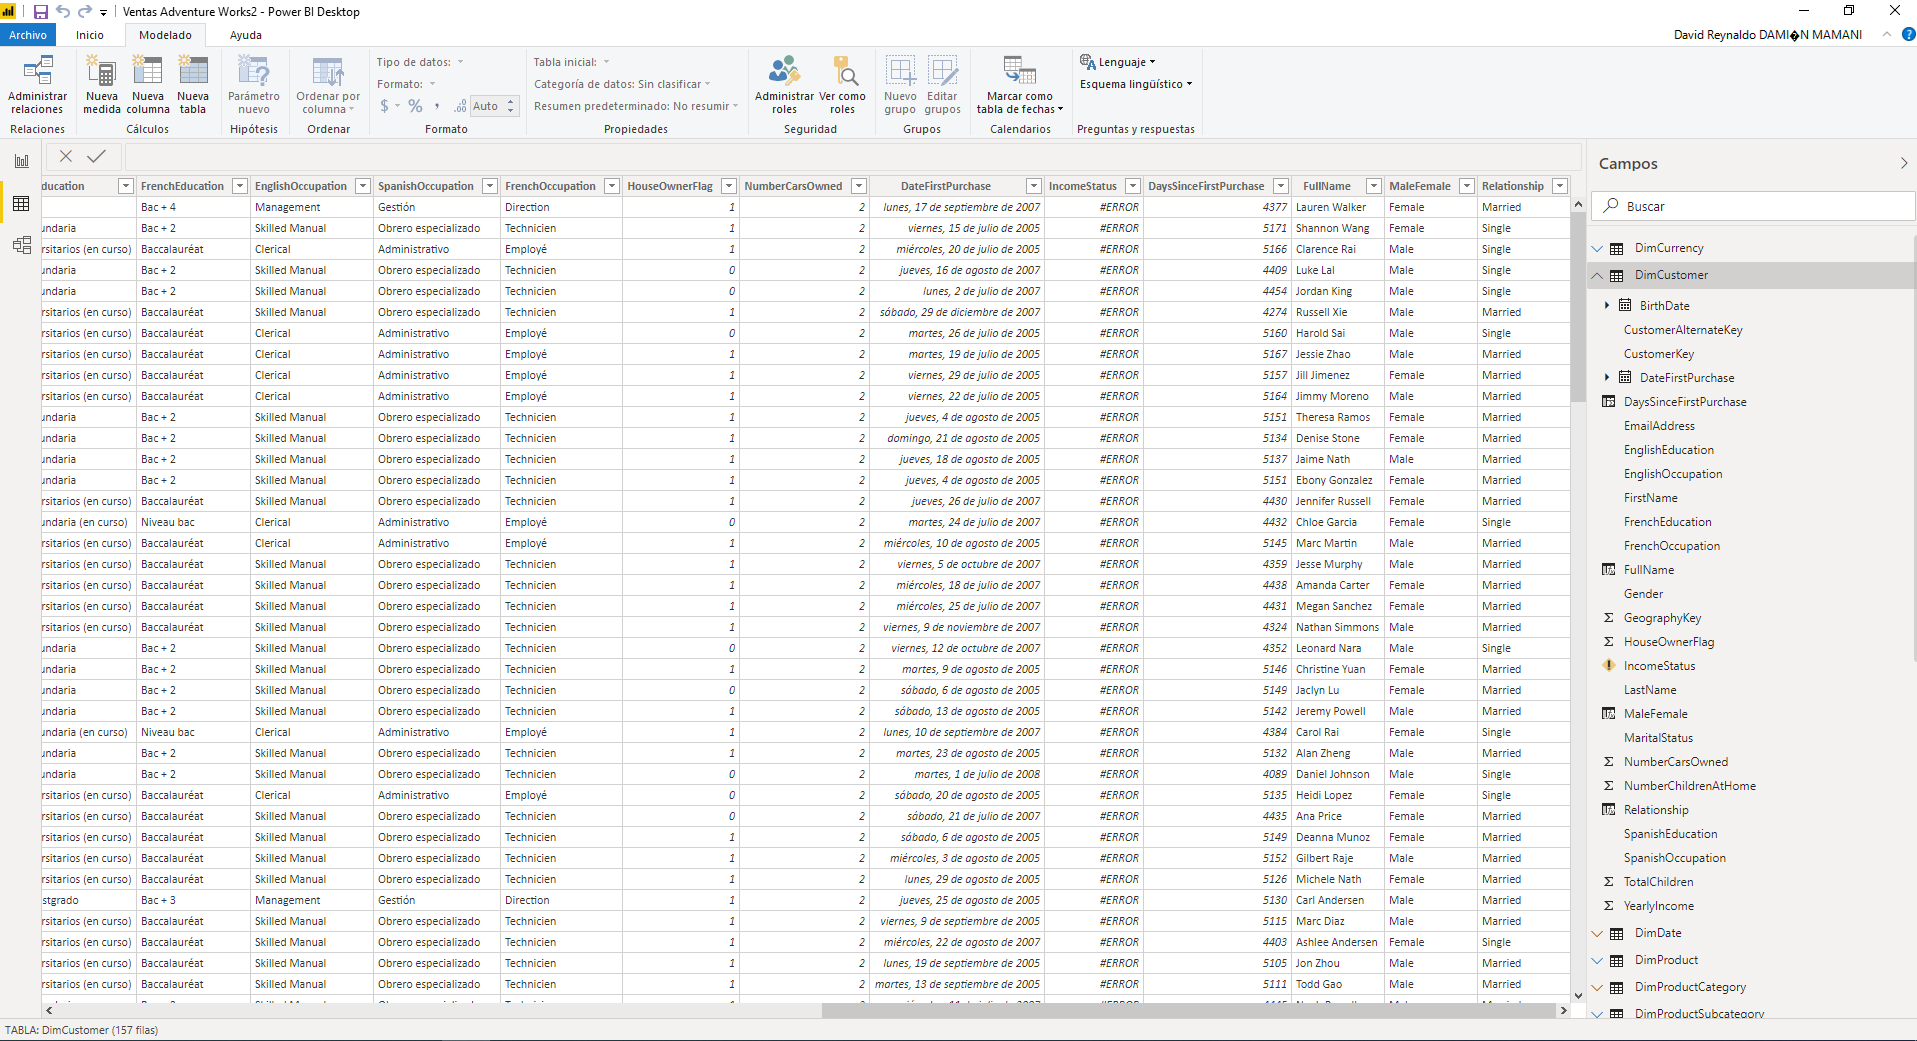
\includegraphics[width=18cm]{./Imagenes/Imagen3}
	\end{center}	
\end{itemize}

\subsection {Construyendo Reportes en Power BI}







